\documentclass{standalone}
\usepackage{tikz}
\usetikzlibrary{patterns, positioning}

\begin{document}
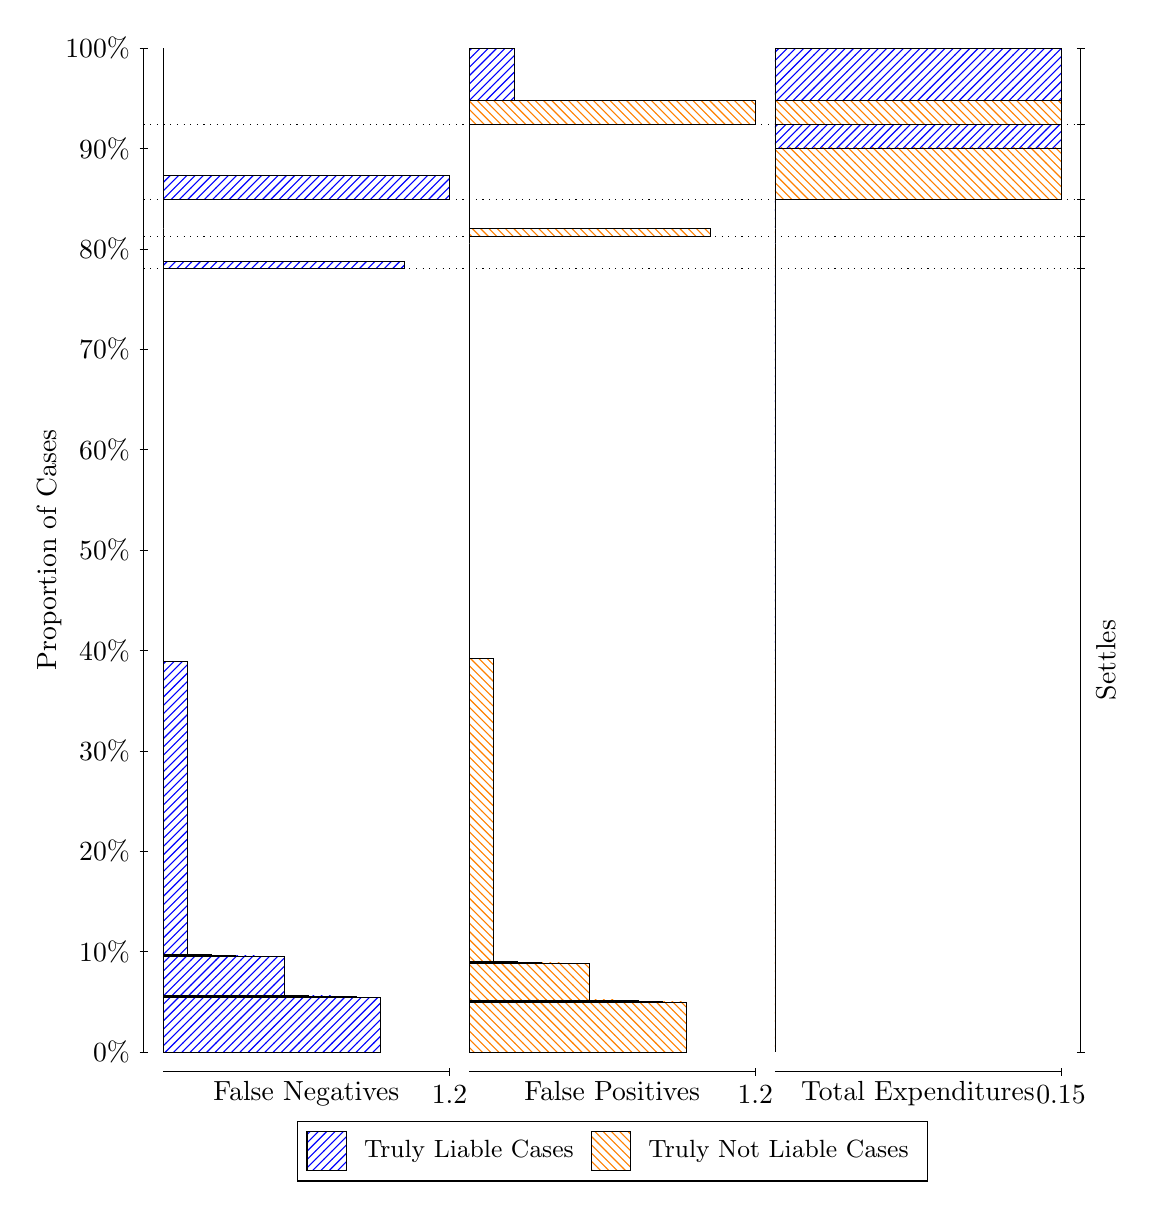
\begin{tikzpicture}
\draw[black, very thin] (1.5,1.75) -- (1.5,14.5);
\node[rotate=90, anchor=center] at (0.3, 8.125) {Proportion of Cases};
\draw[black, very thin] (1.45,1.75) -- (1.55,1.75);
\node[anchor=east] at (1.45, 1.75) {0\%};
\draw[black, very thin] (1.45,3.025) -- (1.55,3.025);
\node[anchor=east] at (1.45, 3.025) {10\%};
\draw[black, very thin] (1.45,4.3) -- (1.55,4.3);
\node[anchor=east] at (1.45, 4.3) {20\%};
\draw[black, very thin] (1.45,5.575) -- (1.55,5.575);
\node[anchor=east] at (1.45, 5.575) {30\%};
\draw[black, very thin] (1.45,6.85) -- (1.55,6.85);
\node[anchor=east] at (1.45, 6.85) {40\%};
\draw[black, very thin] (1.45,8.125) -- (1.55,8.125);
\node[anchor=east] at (1.45, 8.125) {50\%};
\draw[black, very thin] (1.45,9.4) -- (1.55,9.4);
\node[anchor=east] at (1.45, 9.4) {60\%};
\draw[black, very thin] (1.45,10.675) -- (1.55,10.675);
\node[anchor=east] at (1.45, 10.675) {70\%};
\draw[black, very thin] (1.45,11.95) -- (1.55,11.95);
\node[anchor=east] at (1.45, 11.95) {80\%};
\draw[black, very thin] (1.45,13.225) -- (1.55,13.225);
\node[anchor=east] at (1.45, 13.225) {90\%};
\draw[black, very thin] (1.45,14.5) -- (1.55,14.5);
\node[anchor=east] at (1.45, 14.5) {100\%};

\draw[black, very thin] (13.4,1.75) -- (13.4,14.5);
\draw[black, very thin] (13.35,1.75) -- (13.45,1.75);
\node[anchor=west] at (13.35, 1.75) {};
\draw[black, very thin] (13.35,11.703) -- (13.45,11.703);
\node[anchor=west] at (13.35, 11.703) {};
\draw[black, very thin] (13.35,12.104) -- (13.45,12.104);
\node[anchor=west] at (13.35, 12.104) {};
\draw[black, very thin] (13.35,12.577) -- (13.45,12.577);
\node[anchor=west] at (13.35, 12.577) {};
\draw[black, very thin] (13.35,13.534) -- (13.45,13.534);
\node[anchor=west] at (13.35, 13.534) {};
\draw[black, very thin] (13.35,14.5) -- (13.45,14.5);
\node[anchor=west] at (13.35, 14.5) {};

\draw[black, very thin, pattern color=blue, pattern=north east lines] (1.75,1.75) rectangle (4.5037,2.4412);
\draw[black, very thin, pattern color=blue, pattern=north east lines] (1.75,2.4412) rectangle (4.1977,2.4515);
\draw[black, very thin, pattern color=blue, pattern=north east lines] (1.75,2.4515) rectangle (3.8918,2.4623);
\draw[black, very thin, pattern color=blue, pattern=north east lines] (1.75,2.4623) rectangle (3.5858,2.4733);
\draw[black, very thin, pattern color=blue, pattern=north east lines] (1.75,2.4733) rectangle (3.5858,2.4735);
\draw[black, very thin, pattern color=blue, pattern=north east lines] (1.75,2.4735) rectangle (3.2798,2.9611);
\draw[black, very thin, pattern color=blue, pattern=north east lines] (1.75,2.9611) rectangle (2.9739,2.9692);
\draw[black, very thin, pattern color=blue, pattern=north east lines] (1.75,2.9692) rectangle (2.6679,2.9776);
\draw[black, very thin, pattern color=blue, pattern=north east lines] (1.75,2.9776) rectangle (2.3619,2.986);
\draw[black, very thin, pattern color=blue, pattern=north east lines] (1.75,2.986) rectangle (2.056,6.7094);
\draw[black, very thin, pattern color=orange, pattern=north west lines] (1.75,6.7094) rectangle (1.75,11.703);
\draw[black, very thin, pattern color=blue, pattern=north east lines] (1.75,11.703) rectangle (4.8096,11.787);
\draw[black, very thin, pattern color=orange, pattern=north west lines] (1.75,11.787) rectangle (1.75,12.104);
\draw[black, very thin, pattern color=orange, pattern=north west lines] (1.75,12.104) rectangle (1.75,12.211);
\draw[black, very thin, pattern color=blue, pattern=north east lines] (1.75,12.211) rectangle (1.75,12.577);
\draw[black, very thin, pattern color=blue, pattern=north east lines] (1.75,12.577) rectangle (5.3833,12.881);
\draw[black, very thin, pattern color=orange, pattern=north west lines] (1.75,12.881) rectangle (1.75,13.534);
\draw[black, very thin, pattern color=orange, pattern=north west lines] (1.75,13.534) rectangle (1.75,13.838);
\draw[black, very thin, pattern color=blue, pattern=north east lines] (1.75,13.838) rectangle (1.75,14.5);
\draw[black, very thin, pattern color=orange, pattern=north west lines] (5.6333,1.75) rectangle (8.387,2.3851);
\draw[black, very thin, pattern color=orange, pattern=north west lines] (5.6333,2.3851) rectangle (8.0811,2.3944);
\draw[black, very thin, pattern color=orange, pattern=north west lines] (5.6333,2.3944) rectangle (7.7751,2.4036);
\draw[black, very thin, pattern color=orange, pattern=north west lines] (5.6333,2.4036) rectangle (7.4691,2.4126);
\draw[black, very thin, pattern color=orange, pattern=north west lines] (5.6333,2.4126) rectangle (7.1632,2.8721);
\draw[black, very thin, pattern color=orange, pattern=north west lines] (5.6333,2.8721) rectangle (6.8572,2.8723);
\draw[black, very thin, pattern color=orange, pattern=north west lines] (5.6333,2.8723) rectangle (6.8572,2.8818);
\draw[black, very thin, pattern color=orange, pattern=north west lines] (5.6333,2.8818) rectangle (6.5512,2.8911);
\draw[black, very thin, pattern color=orange, pattern=north west lines] (5.6333,2.8911) rectangle (6.2453,2.9);
\draw[black, very thin, pattern color=orange, pattern=north west lines] (5.6333,2.9) rectangle (5.9393,6.7439);
\draw[black, very thin, pattern color=blue, pattern=north east lines] (5.6333,6.7439) rectangle (5.6333,11.703);
\draw[black, very thin, pattern color=orange, pattern=north west lines] (5.6333,11.703) rectangle (5.6333,12.019);
\draw[black, very thin, pattern color=blue, pattern=north east lines] (5.6333,12.019) rectangle (5.6333,12.104);
\draw[black, very thin, pattern color=orange, pattern=north west lines] (5.6333,12.104) rectangle (8.693,12.211);
\draw[black, very thin, pattern color=blue, pattern=north east lines] (5.6333,12.211) rectangle (5.6333,12.577);
\draw[black, very thin, pattern color=orange, pattern=north west lines] (5.6333,12.577) rectangle (5.6333,13.231);
\draw[black, very thin, pattern color=blue, pattern=north east lines] (5.6333,13.231) rectangle (5.6333,13.534);
\draw[black, very thin, pattern color=orange, pattern=north west lines] (5.6333,13.534) rectangle (9.2667,13.838);
\draw[black, very thin, pattern color=blue, pattern=north east lines] (5.6333,13.838) rectangle (6.207,14.5);
\draw[black, very thin, pattern color=orange, pattern=north west lines] (9.5167,1.75) rectangle (9.5167,6.7439);
\draw[black, very thin, pattern color=blue, pattern=north east lines] (9.5167,6.7439) rectangle (9.5167,11.703);
\draw[black, very thin, pattern color=orange, pattern=north west lines] (9.5167,11.703) rectangle (9.5167,12.019);
\draw[black, very thin, pattern color=blue, pattern=north east lines] (9.5167,12.019) rectangle (9.5167,12.104);
\draw[black, very thin, pattern color=orange, pattern=north west lines] (9.5167,12.104) rectangle (9.5167,12.211);
\draw[black, very thin, pattern color=blue, pattern=north east lines] (9.5167,12.211) rectangle (9.5167,12.577);
\draw[black, very thin, pattern color=orange, pattern=north west lines] (9.5167,12.577) rectangle (13.15,13.231);
\draw[black, very thin, pattern color=blue, pattern=north east lines] (9.5167,13.231) rectangle (13.15,13.534);
\draw[black, very thin, pattern color=orange, pattern=north west lines] (9.5167,13.534) rectangle (13.15,13.838);
\draw[black, very thin, pattern color=blue, pattern=north east lines] (9.5167,13.838) rectangle (13.15,14.5);
\draw[black, dotted] (1.5,11.703) -- (13.4,11.703);
\draw[black, dotted] (1.5,12.104) -- (13.4,12.104);
\draw[black, dotted] (1.5,12.577) -- (13.4,12.577);
\draw[black, dotted] (1.5,13.534) -- (13.4,13.534);
\draw[black, very thin] (1.75,1.5) -- (5.3833,1.5);
\node[anchor=north] at (3.5667, 1.5) {False Negatives};
\draw[black, very thin] (5.3833,1.45) -- (5.3833,1.55);
\node[anchor=north] at (5.3833, 1.45) {1.2};

\draw[black, very thin] (5.6333,1.5) -- (9.2667,1.5);
\node[anchor=north] at (7.45, 1.5) {False Positives};
\draw[black, very thin] (9.2667,1.45) -- (9.2667,1.55);
\node[anchor=north] at (9.2667, 1.45) {1.2};

\draw[black, very thin] (9.5167,1.5) -- (13.15,1.5);
\node[anchor=north] at (11.333, 1.5) {Total Expenditures};
\draw[black, very thin] (13.15,1.45) -- (13.15,1.55);
\node[anchor=north] at (13.15, 1.45) {0.15};

\node[black, centered, rotate=90] at (13.72, 6.7266) {Settles};





\draw (7.449999999999999,1.5) node[draw=none] (baseCoordinate) {};
\begin{scope}[align=center]
        \matrix[scale=0.5, draw=black, below=0.5cm of baseCoordinate, nodes={draw}, column sep=0.1cm]{
            \node[rectangle, draw, minimum width=0.5cm, minimum height=0.5cm, pattern=north east lines, pattern color=blue] {}; &
            \node[draw=none, font=\small] (B) {Truly Liable Cases}; &
            \node[rectangle, draw, minimum width=0.5cm, minimum height=0.5cm, pattern=north west lines, pattern color=orange] {}; &
            \node[draw=none, font=\small] (B) {Truly Not Liable Cases}; \\
            };
\end{scope}

\end{tikzpicture}
\end{document}